% Electronic Supplementary Material (ESM) for main.tex.
% Built from the material moved out of the main text in the length
% reduction (paper/LENGTH_PLAN.md). Compile separately.
\documentclass[11pt]{article}
\usepackage[T1]{fontenc}
\usepackage{amsmath,amssymb}
\usepackage{graphicx}
\usepackage{booktabs}
\usepackage[margin=2.5cm]{geometry}
\usepackage{hyperref}
\renewcommand{\thesection}{S\arabic{section}}
\renewcommand{\thetable}{S\arabic{table}}
\renewcommand{\thefigure}{S\arabic{figure}}
\title{Supplementary Material for ``Confidence Aggregation in Closed-Loop
Information Extraction: Formal Analysis and Empirical Evaluation''}
\date{}
\begin{document}
\maketitle

\section{Extended Experimental Setup}
\label{sec:s1}

This section gives the rationale and procedural detail behind the setup
in the main text's Experimental Setup section.

\paragraph{CaRB sample.} The 548 CaRB test sentences are those whose text
matches between \texttt{data/CaRB/data/test.txt} and the gold annotation
file \texttt{test.tsv} by exact string. The 93 excluded sentences differ
between the two files in whitespace and quoting; the exclusion is a
pre-existing mismatch, not a selection. The official CaRB scorer's AUC is
a single-point approximation, since the extractors produce one operating
point rather than a confidence-ranked list.

\paragraph{Comparison systems.} \texttt{Babelscape/rebel-large} was
attempted as a CaRB comparison system and found incompatible with CaRB's
open-domain, span-based scoring: REBEL is a closed, Wikidata-schema
relation extractor, so its raw score against CaRB's scorer is not a
meaningful comparison and is not reported. GPT-4o, Claude Sonnet 5 and
Gemini 2.5 Pro were evaluated on the original 30-sentence CaRB pilot
only; Gemini 2.5 Pro needed a 3,072-token output budget and still
returned no valid output for 5 of the 30 sentences. GenIE, InstructUIE, DyGIE++, and TACRED were outside the scope of this evaluation.

\paragraph{Fine-tuning base model and hardware.}
Mistral-7B-Instruct-v0.3 was chosen over Llama-3.1-8B-Instruct to avoid
a gated-repository approval wait. Training and adapter evaluation ran on
rented RunPod GPUs, mostly an RTX 4090 (24 GB), with an RTX 3090
substituted for some runs after RTX 4090 pods failed GPU sanity checks;
runtime is not compared across GPU types.

\paragraph{Why DocRED and BioRED use $\lambda=0.5$, $\tau=0.70$.} Under
$\lambda=0.5$, the product-domain threshold $\tau=0.88$ would require
four or more corroborating observations (the argument of the
corroboration-requirement proposition with these values), which the
public corpora's evidence structure rarely supplies; $\tau=0.70$ is
reachable with two. The values were set for the DocRED pilot and kept
fixed, not tuned.

\paragraph{The Wilcoxon floor at five seeds.} With $n=5$, the Wilcoxon
signed-rank test cannot report $p$ below $0.0625$, the value reached
when all five paired differences share a sign. A Wilcoxon $p=0.0625$ at
five seeds is therefore the strongest result the test can give, not a
weaker one than an accompanying $t$-test.

\paragraph{Recall denominators in detail.} DEC-026's recall uses the
\texttt{gold\_unstructured} facts of train-split products, built with the
same \texttt{normalize\_gold()} logic as the original run scripts, and
matching the snapshots' own \texttt{gold\_label} column with zero
mismatches on both snapshots. It is directly comparable to EVID-014's
admission recall on the same 657-triple snapshot at $\tau=0.88$. It is
not comparable to the held-out extraction recall of EVID-013, which is
measured on other products from a single extraction pass with no
admission step, or to the closed-loop test's recall, which uses the
larger \texttt{gold\_structured} set (checked against
\texttt{scripts/dec019\_closedloop\_compare.py}).

\paragraph{DEC-026 cost.} DEC-026 is a replay of knowledge-base snapshots
saved by the product-domain runs: it re-scores stored observations under
six rules, with no API calls or GPU time.

\section{Aggregation-Rule Comparison: Full Tables}
\label{sec:s2}

Full results of the offline replay (DEC-026) summarised in the main text's Section on empirical validation of the aggregation rule. Rules: R1 max-merge; R2 the published rule; R3 distinct-source counting; R4 evidence share; R5 R3 and R4 combined; R6 the unsquared share (exploratory). Dataset A: 657 triples, 35 test-split subjects; dataset B: 2,241 triples, 92.

\begin{table}[htbp]
\centering
\caption{Dataset A (657 triples): precision, recall, and $F_1$ at each
rule's own F1-selected threshold and at the fixed $\tau=0.88$, side by
side.}
\label{tab:dec026-a-metrics}
\begin{tabular}{@{}lc ccc ccc@{}}
\toprule
& & \multicolumn{3}{c}{F1-selected} & \multicolumn{3}{c}{Fixed $\tau=0.88$} \\
\cmidrule(lr){3-5} \cmidrule(lr){6-8}
Rule & $\tau_{\text{sel}}$ & $P$ & $R$ & $F_1$ & $P$ & $R$ & $F_1$ \\
\midrule
R1 (max-merge) & 0.98 & 0.5385 & 1.0000 & 0.7000 & 0.4389 & 1.0000 & 0.6100 \\
R2 (published) & 0.73 & 0.5095 & 0.9571 & 0.6650 & 0.8333 & 0.3929 & 0.5340 \\
R3 (source-count) & 0.73 & 0.5214 & 0.9571 & 0.6751 & 0.9322 & 0.3929 & 0.5528 \\
R4 (evidence-share) & 0.73 & 0.5095 & 0.9571 & 0.6650 & 0.8333 & 0.3929 & 0.5340 \\
R5 (R3+R4) & 0.73 & 0.5214 & 0.9571 & 0.6751 & 0.9322 & 0.3929 & 0.5528 \\
R6 (unsquared, exploratory) & 0.73 & 0.4621 & 0.9571 & 0.6233 & 0.4674 & 0.9214 & 0.6202 \\
\bottomrule
\end{tabular}
% [EVID-041]
\end{table}

\begin{table}[htbp]
\centering
\caption{Dataset B (2241 triples): precision, recall, and $F_1$ at each
rule's own F1-selected threshold and at the fixed $\tau=0.88$, side by
side.}
\label{tab:dec026-b-metrics}
\begin{tabular}{@{}lc ccc ccc@{}}
\toprule
& & \multicolumn{3}{c}{F1-selected} & \multicolumn{3}{c}{Fixed $\tau=0.88$} \\
\cmidrule(lr){3-5} \cmidrule(lr){6-8}
Rule & $\tau_{\text{sel}}$ & $P$ & $R$ & $F_1$ & $P$ & $R$ & $F_1$ \\
\midrule
R1 (max-merge) & 0.98 & 0.5308 & 1.0000 & 0.6935 & 0.4481 & 1.0000 & 0.6188 \\
R2 (published) & 0.73 & 0.5102 & 0.9317 & 0.6593 & 0.9012 & 0.4534 & 0.6033 \\
R3 (source-count) & 0.73 & 0.5149 & 0.9317 & 0.6632 & 0.9280 & 0.4534 & 0.6092 \\
R4 (evidence-share) & 0.73 & 0.5102 & 0.9317 & 0.6593 & 0.9012 & 0.4534 & 0.6033 \\
R5 (R3+R4) & 0.73 & 0.5149 & 0.9317 & 0.6632 & 0.9280 & 0.4534 & 0.6092 \\
R6 (unsquared, exploratory) & 0.58 & 0.4894 & 0.9524 & 0.6465 & 0.5023 & 0.8986 & 0.6444 \\
\bottomrule
\end{tabular}
% [EVID-041]
\end{table}

\begin{table}[htbp]
\centering
\caption{Admitted-triple counts and contested single-valued-predicate
slots with at least one candidate admitted, both datasets, both
thresholds.}
\label{tab:dec026-admitted}
\begin{tabular}{@{}llcc cc@{}}
\toprule
& & \multicolumn{2}{c}{F1-selected} & \multicolumn{2}{c}{Fixed $\tau=0.88$} \\
\cmidrule(lr){3-4} \cmidrule(lr){5-6}
Dataset & Rule & Admitted & Contested slots & Admitted & Contested slots \\
\midrule
A (657) & R1 & 260 & 6 & 319 & 20 \\
A (657) & R2 & 263 & 0 & 66 & 0 \\
A (657) & R3 & 257 & 0 & 59 & 0 \\
A (657) & R4 & 263 & 0 & 66 & 0 \\
A (657) & R5 & 257 & 0 & 59 & 0 \\
A (657) & R6 & 290 & 0 & 276 & 0 \\
\midrule
B (2241) & R1 & 910 & 40 & 1078 & 69 \\
B (2241) & R2 & 882 & 0 & 243 & 0 \\
B (2241) & R3 & 874 & 0 & 236 & 0 \\
B (2241) & R4 & 882 & 0 & 243 & 0 \\
B (2241) & R5 & 874 & 0 & 236 & 0 \\
B (2241) & R6 & 940 & 10 & 864 & 0 \\
\bottomrule
\end{tabular}
% [EVID-041]
\end{table}

\begin{table}[htbp]
\centering
\caption{Bootstrap 95\% CI for $F_1(\text{rule}) - F_1(\text{R2})$ at
each rule's own F1-selected threshold, $10{,}000$ resamples over
test-split subjects.}
\label{tab:dec026-bootstrap-f1sel}
\begin{tabular}{@{}llrrc@{}}
\toprule
Dataset & Rule & Mean diff. & 95\% CI & Excludes 0 \\
\midrule
A (657) & R1 & $+0.0359$ & $[0.0154, 0.0641]$ & Yes \\
A (657) & R3 & $+0.0106$ & $[0.0028, 0.0222]$ & Yes \\
A (657) & R4 & $+0.0000$ & $[0.0000, 0.0000]$ & No \\
A (657) & R5 & $+0.0106$ & $[0.0028, 0.0222]$ & Yes \\
A (657) & R6 & $-0.0429$ & $[-0.0870, -0.0118]$ & Yes \\
\midrule
B (2241) & R1 & $+0.0341$ & $[0.0191, 0.0496]$ & Yes \\
B (2241) & R3 & $+0.0039$ & $[0.0013, 0.0075]$ & Yes \\
B (2241) & R4 & $+0.0000$ & $[0.0000, 0.0000]$ & No \\
B (2241) & R5 & $+0.0039$ & $[0.0013, 0.0075]$ & Yes \\
B (2241) & R6 & $-0.0131$ & $[-0.0303, 0.0015]$ & No \\
\bottomrule
\end{tabular}
% [EVID-041]
\end{table}


\section{Computational Complexity}
\label{sec:formal-analysis-complexity}

The production candidate-acceptance path is empirically $O(N)$ per call
and $O(N^2)$ cumulative over $N$ accumulated observations
% [EVID-036]
, caused by a linear scan over every previously accepted candidate in
\texttt{src/pkb\_instrumentation.accepted\_slot\_keys} on every new
observation -- measured at $72.7\times$ latency growth for $80\times$
more observations
% [EVID-036]
. An indexed alternative (same aggregation mathematics, keyed by
normalized (subject, predicate) slot rather than scanned linearly)
achieves $O(1)$ per call and $O(N)$ cumulative
% [EVID-036]
; it was implemented illustratively but not wired into the evaluated
system. This is not a limiting factor at the scale evaluated in this
paper ($N$ in the hundreds, the main text's Experimental Setup section), where
LLM API latency dominates wall-clock time
% [EVID-036, cross-referenced against DEC-008's linear end-to-end runtime
% finding]
, but is stated here as a forward-looking scalability property of the
current implementation, separate from the aggregation rule's own
mathematical properties above.


\begin{table}[htbp]
\centering
\caption{Growth in per-call latency of candidate acceptance (100 to
8,000 observations).}
\label{tab:s8-complexity}
\begin{tabular}{@{}lcc@{}}
\toprule
Implementation & Growth in observations & Growth in per-call latency \\
\midrule
Production routine (linear scan over accepted candidates) & 80$\times$ & 72.7$\times$ \\
Indexed variant (benchmark only, not in pipeline) & 80$\times$ & 2.9$\times$ \\
\bottomrule
\end{tabular}
% [EVID-036]
\end{table}

\section{Module Ablation: Five-Seed Runs}
\label{sec:s4}

Before the thirty-seed extension, the ablation was run at five seeds
($42$--$46$) at $N=20$ (4 held-out test products) and $N=50$ (10), with
five configurations: the full pipeline, without the feedback controller,
without the probabilistic knowledge base (max-merge), structured-only,
and unstructured-only (Table~\ref{tab:s3-ablation-full}). Neither
ablated variant differed significantly from the full pipeline at either
scale (all $p \ge 0.31$). The direction for the variant without the
feedback controller reversed between scales ($+0.142$ at $N=20$;
$-0.045$ at $N=50$), whereas the max-merge variant scored higher than
the full pipeline at both ($+0.147$; $+0.033$). With five seeds, a paired
$t$-test has 80\% power only for standardised effects of about $1.7$
standard deviations, about $0.29$ absolute $F_1$ at the observed
variance, so these runs rule out only large effects. The structured-only
and unstructured-only variants have no held-out evaluation by design.
% [EVID-020; EVID-039; AUDIT.md]

\paragraph{Standard-deviation correction.} EVID-039 logged these $F_1$
standard deviations as population SDs ($\text{ddof}=0$), e.g.\ $0.0934$
for the full pipeline's held-out $F_1$. The values in
Table~\ref{tab:s3-ablation-full} are converted to sample SDs
($\times\sqrt{n/(n-1)}$, $n=5$; $0.0934 \times \sqrt{5/4} = 0.104$),
matching the project's $\text{ddof}=1$ convention. No mean,
$t$-statistic, or $p$-value changes; only the SD figures do. The same
correction applies to the five-epoch fine-tuning SD in
Section~\ref{sec:s5}.

\begin{table}[htbp]
\centering
\caption{Five-seed ablation results at $N=20$ and $N=50$: mean (SD)
and paired comparisons with the full pipeline (the thirty-seed $N=50$
result is in the main text's thirty-seed ablation table).}
\label{tab:s3-ablation-full}
\begin{tabular}{@{}lll@{}}
\toprule
Configuration / comparison & $N=20$ & $N=50$ \\
\midrule
\multicolumn{3}{@{}l}{\emph{Held-out test $F_1$}} \\
Full pipeline & 0.2914 (0.3349) & 0.3451 (0.1044) \\
Without feedback controller & 0.4335 (0.1833) & 0.3005 (0.1932) \\
Without PKB (max-merge) & 0.4388 (0.2866) & 0.3783 (0.1950) \\
$\Delta$ without feedback [95\% CI]; $p$ ($t$/Wilcoxon) & $+0.142\ [-0.400, 0.684]$; $0.507/0.438$ & $-0.045\ [-0.245, 0.156]$; $0.571/0.625$ \\
$\Delta$ without PKB [95\% CI]; $p$ ($t$/Wilcoxon) & $+0.147\ [-0.297, 0.592]$; $0.409/0.438$ & $+0.033\ [-0.146, 0.213]$; $0.635/1.000$ \\
\multicolumn{3}{@{}l}{\emph{Training $F_1$}} \\
Full pipeline & 0.4233 (0.1379) & 0.4070 (0.1206) \\
Without feedback controller & 0.2878 (0.1867) & 0.3328 (0.0464) \\
Without PKB (max-merge) & 0.3437 (0.1258) & 0.3761 (0.1372) \\
Unstructured only & 0.4572 (0.0987) & 0.4478 (0.0884) \\
$\Delta$ without feedback [95\% CI]; $p$ ($t$/Wilcoxon) & $-0.136\ [-0.536, 0.265]$; $0.400/0.438$ & $-0.074\ [-0.266, 0.118]$; $0.343/0.313$ \\
$\Delta$ without PKB [95\% CI]; $p$ ($t$/Wilcoxon) & $-0.080\ [-0.291, 0.132]$; $0.354/0.313$ & $-0.031\ [-0.245, 0.183]$; $0.709/0.813$ \\
\bottomrule
\end{tabular}

\noindent\emph{Note.} $N=20$ used 4 held-out test products and $N=50$
used 10. $N=50$ SDs are sample SDs converted from the logged population
SDs (Section~\ref{sec:s4}); $N=20$ SDs
are as logged. CIs are derived from logged mean differences and paired
$p$-values. The structured-only variant has no LLM component and was
not scored.
% [EVID-020; EVID-039]
\end{table}

\section{Superseded Fine-Tuning Exploration (Tuned on Its Own Test Set)}
\label{sec:s5}

\textbf{The results in this section are superseded by the leakage-free,
pre-registered evaluation in the main text (Automated Fine-Tuning Evaluation), which is
negative, and are not a current finding.} They selected hyperparameters
and then tested significance on the same 8-product test set.

\paragraph{The tuning-leakage issue and its resolution.} The epoch and
LoRA grid that selected the 5-epoch configuration, and the five-seed
run that reported $p=0.0028$ for it, both evaluated on the same 8-product
test split. It has 8 products rather than 10 because an automated
leakage guard excludes any test product whose name appears in the
fine-tuning data, and excludes 2 of the 10. There was no independent
validation split separating selection from confirmation. DEC-024
pre-registered the fix (select on the 200-product superset's 20-product
validation split, confirm once on its untouched 40-product test split),
executed as DEC-027 with a leakage-guard unit test
(\texttt{tests/test\_dec027\_leakage\_guard.py}) that aborts training
before any GPU time is spent if a held-out product appears in the
training data. The one-sample tests below also treat the base score as
fixed, so they capture variation across training seeds but not across
test products, of which there were only 8 (7 base-model true
positives).
% [scripts/dec006_evaluate_adapter.py; EVID-037; Decision log.md, DEC-024, DEC-027; EVID-044]

\paragraph{Results.} Mistral-7B-Instruct-v0.3 was fine-tuned with QLoRA
on the same 90 synthetic examples. The base model (greedy decoding)
predicted 46 triples, 7 of them correct ($P=0.152$, $R=0.125$,
$F_1=0.137$). An earlier evaluation in which two intended test products
also appeared in the training data was withdrawn, and both products
were excluded.
% [EVID-026; EVID-027; EVID-028]
In a seed-42 search, precision increased with training epochs, reaching
$1.000$ at 5 and 8 epochs, while recall stayed at $0.125$
(Figure~\ref{fig:finetuning}a; Table~\ref{tab:s4-epoch-search}). No
alternative LoRA rank or learning rate exceeded the default configuration
(Table~\ref{tab:s5-lora-search}), and recall was $0.125$ in all nine
runs. \textbf{This flat recall does not show that fine-tuning leaves
recall unchanged}: the base model found only 7 of 56 gold triples, so a
loss of about 10\% of true positives, the size measured in DEC-027, is
less than one triple and could not appear on this set. Over five seeds
(Table~\ref{tab:finetune-5seed}; Figure~\ref{fig:finetuning}b), with the
configuration tuned on the same test set, the 5-epoch configuration
exceeded the base model in every seed ($\Delta F_1=+0.064$, 95\% CI
$[0.037,0.091]$, $t(4)=6.57$, $p=0.003$), and the 3-epoch configuration
in four of five ($+0.044$, $[-0.005,0.093]$, $p=0.066$); the two did not
differ significantly ($+0.020$, $[-0.045,0.085]$, $p=0.446$).
% [EVID-037; EVID-038; EVID-040]

\begin{table}[htbp]
\centering
\caption{Five-seed fine-tuning results on the earlier 8-product test set, with hyperparameters tuned on that same test set (historical; superseded by the negative result in the main text's leakage-free fine-tuning table).}
\label{tab:finetune-5seed}
\begin{tabular}{@{}lrrrrrr@{}}
\toprule
Configuration & $F_1$, mean (SD) & $\Delta F_1$ [95\% CI] & $t(4)$ & $p$ & Wilcoxon $p$ & Seeds $>$ base \\
\midrule
Base model & 0.137 & --- & --- & --- & --- & --- \\
3 epochs & 0.181 (0.039) & $+0.044\ [-0.005, 0.093]$ & 2.51 & 0.066 & 0.125 & 4/5 \\
5 epochs & 0.201 (0.022) & $+0.064\ [0.037, 0.091]$ & 6.57 & 0.003 & 0.063 & 5/5 \\
5 vs.\ 3 epochs (paired) & --- & $+0.020\ [-0.045, 0.085]$ & 0.84 & 0.446 & 0.625 & --- \\
\bottomrule
\end{tabular}
% [EVID-040; SD corrected to sample SD, see the note in
% Section~\ref{sec:s4} -- EVID-040's logged 0.0194 for the
% 5-epoch configuration is the population SD; the sample SD is 0.0217,
% independently recomputed this session from the per-seed values in
% Table~\ref{tab:s6-per-seed} and confirmed to match ($t(4)=6.57$ is
% consistent only with the sample-SD figure, not 0.0194]
\end{table}

\begin{figure}[htbp]
\centering
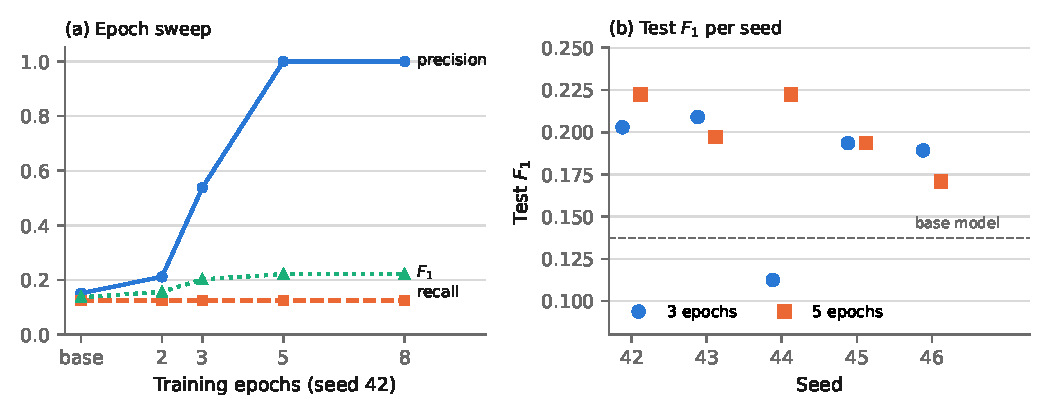
\includegraphics[width=0.9\linewidth]{figures/fig_finetuning.pdf}
\caption{Earlier, tuning-leakage-affected fine-tuning exploration
(superseded; the main text's leakage-free fine-tuning table is the headline result). (a) Precision, recall, and $F_1$ against training
epochs (seed 42). (b) Test $F_1$ per seed for the 3- and 5-epoch
configurations; the dashed line marks the base model.}
\label{fig:finetuning}
% [SLDE-AFT_Section7_Results_revised.docx, Figure 7.3]
\end{figure}

\begin{table}[htbp]
\centering
\caption{Epoch search (seed 42; rank 16, $\alpha=32$, learning rate
$2\times10^{-4}$; 8-product test set).}
\label{tab:s4-epoch-search}
\begin{tabular}{@{}lccc@{}}
\toprule
Configuration & $P$ & $R$ & $F_1$ \\
\midrule
Base model & 0.1522 & 0.1250 & 0.1373 \\
2 epochs & 0.2121 & 0.1250 & 0.1573 \\
3 epochs & 0.5385 & 0.1250 & 0.2029 \\
5 epochs & 1.0000 & 0.1250 & 0.2222 \\
8 epochs & 1.0000 & 0.1250 & 0.2222 \\
\bottomrule
\end{tabular}
% [EVID-037]
\end{table}

\begin{table}[htbp]
\centering
\caption{LoRA hyperparameter search at 5 epochs (seed 42; 8-product test set).}
\label{tab:s5-lora-search}
\begin{tabular}{@{}lccc@{}}
\toprule
Setting & $P$ & $R$ & $F_1$ \\
\midrule
Rank 8, $\alpha=16$, lr $2\times10^{-4}$ & 0.7778 & 0.1250 & 0.2154 \\
Rank 16, $\alpha=32$, lr $2\times10^{-4}$ (default) & 1.0000 & 0.1250 & 0.2222 \\
Rank 32, $\alpha=64$, lr $2\times10^{-4}$ & 0.7000 & 0.1250 & 0.2121 \\
Rank 16, $\alpha=32$, lr $1\times10^{-4}$ & 0.2258 & 0.1250 & 0.1609 \\
Rank 16, $\alpha=32$, lr $3\times10^{-4}$ & 0.3684 & 0.1250 & 0.1867 \\
\bottomrule
\end{tabular}
% [EVID-038]
\end{table}

\begin{table}[htbp]
\centering
\caption{Per-seed test $F_1$ at 3 and 5 epochs (8-product test set;
base model $F_1=0.1373$).}
\label{tab:s6-per-seed}
\begin{tabular}{@{}lcc@{}}
\toprule
Seed & 3 epochs & 5 epochs ($P$ / $R$ / $F_1$) \\
\midrule
42 & 0.2029 & 1.0000 / 0.1250 / 0.2222 \\
43 & 0.2090 & 0.4667 / 0.1250 / 0.1972 \\
44 & 0.1124 & 1.0000 / 0.1250 / 0.2222 \\
45 & 0.1935 & 1.0000 / 0.1071 / 0.1935 \\
46 & 0.1892 & 0.2692 / 0.1250 / 0.1707 \\
Mean (sample SD) & 0.1814 (0.0393) & 0.2012 (0.0217) \\
\bottomrule
\end{tabular}
% [EVID-034 (3 epochs); EVID-040 (5 epochs); 5-epoch sample SD
% 0.0217 independently recomputed this session from these per-seed
% values -- EVID-040's logged 0.0194 is the population SD, see
% Section~\ref{sec:s4}]
\end{table}

\section{Scalability}
\label{sec:s6}

For a single unguided extraction pass, total runtime increased
approximately linearly from 92\,s at $N=20$ to 799\,s at $N=200$, and
mean per-document latency stayed between $3.98$ and $4.60$\,s while the
knowledge base grew to 2,814 entries (Figure~\ref{fig:scalability};
Table~\ref{tab:s7-scalability}). Each size was run once, and the full
four-iteration loop was not profiled beyond $N=200$. Memory use could
not be measured reliably, because all sizes ran in one process, and GPU
utilisation during fine-tuning was not recorded.
% [EVID-023]

\begin{figure}[htbp]
\centering
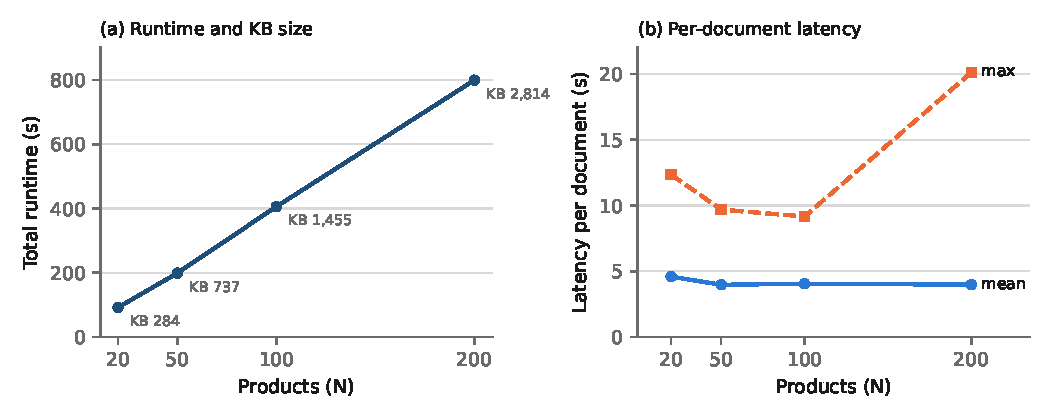
\includegraphics[width=0.9\linewidth]{figures/fig_scalability.pdf}
\caption{Scalability of a single unguided extraction pass (seed 42):
(a) total runtime and knowledge-base size; (b) mean and maximum
per-document latency.}
\label{fig:scalability}
% [SLDE-AFT_Section7_Results_revised.docx, Figure 7.4]
\end{figure}

\begin{table}[htbp]
\centering
\caption{Scalability of a single unguided extraction pass (seed 42).}
\label{tab:s7-scalability}
\begin{tabular}{@{}lrrrrrrr@{}}
\toprule
$N$ & Runtime (s) & Mean latency (s) & Max latency (s) & KB size & Conflicts & Above $\tau$ & Failed calls \\
\midrule
20 & 92.14 & 4.598 & 12.35 & 284 & 8 & 37 & 9 (45\%) \\
50 & 199.04 & 3.976 & 9.69 & 737 & 59 & 106 & 17 (34\%) \\
100 & 405.84 & 4.053 & 9.17 & 1,455 & 117 & 263 & 24 (24\%) \\
200 & 799.06 & 3.988 & 20.12 & 2,814 & 187 & 547 & 53 (26.5\%) \\
\bottomrule
\end{tabular}

\noindent\emph{Note.} The failure rate reflects a deliberately unguided
single pass and is not comparable with guided multi-iteration runs.
% [EVID-023]
\end{table}

\section{DocRED and BioRED: Pilot-Continuity Settings}
\label{sec:s7}

These settings reproduce the earlier pilots' conditions on the same
extractions, for comparison with them. They do not decide any
pre-registered verdict.

\paragraph{DocRED, gold evidence sentences only.} Restricting the 845-document
extractions to the 3,918 gold evidence sentences (the 15-document
pilot's oracle setting) gives the same pattern as all sentences: no
aggregation $F_1=0.056$, every PKB arm $F_1 \le 0.005$. Under the
pilot's exact first-mention evaluator, no aggregation scores $F_1=0.030$
(all sentences) and $0.037$ (evidence only). The 15-document pilot had
reported $F_1$ of $0.033$ without and $0.010$ with aggregation.
% [EVID-046; Decision log.md, DEC-020]

\paragraph{BioRED, whole abstracts and pilot evaluators.} Extracting from
each whole abstract in one call (the 15-abstract pilot's setting, with
its six-relation prompt) gives no-aggregation $F_1$ of $0.049$
(Llama-3.1-8B) and $0.089$ (DeepSeek-V3.2); a whole abstract is a single
source, so no aggregation arm applies. At sentence level, the pilot's
relaxed containment evaluator roughly doubles no-aggregation $F_1$
($0.107$ and $0.158$) but barely changes the aggregated arms, whose few
admitted triples mostly match exactly. The 15-abstract pilot had
reported $F_1=0.007$ (strict) and $0.103$ (relaxed).
% [EVID-047; EVID-024]

\section{Calibration Bins and Iteration Metrics}
\label{sec:s8}

Per-bin calibration values for the reliability diagram, and per-iteration extraction metrics for the 50-product run.

\begin{table}[htbp]
\centering
\caption{Calibration bins of conflict-adjusted scores (657 gold-labelled
triples; ECE $=0.3332$, Brier $=0.2969$).}
\label{tab:s1-calibration}
\begin{tabular}{@{}lccc@{}}
\toprule
Confidence bin & Triples & Mean confidence & Fraction correct \\
\midrule
0.6--0.7 & 68 & [add] & 0.000 \\
0.8--0.9 & 16 & [add] & 0.000 \\
0.9--1.0 & 114 & 0.978 & 0.868 \\
Remaining bins & [add] & [add] & [add] \\
\bottomrule
\end{tabular}

\noindent\emph{Note.} Complete from
\texttt{calibration\_bins\_real.csv} before submission (not committed
to this repository).
% [EVID-036; SLDE-AFT_Section7_Supplementary.docx]
\end{table}

\begin{table}[htbp]
\centering
\caption{LLM-only extraction on training products per iteration, and
held-out base-extractor $F_1$ (single seed).}
\label{tab:s2-iteration}
\begin{tabular}{@{}lcccc@{}}
\toprule
Iteration / split & $P$ & $R$ & $F_1$ & KB size \\
\midrule
Iteration 1 (unguided) & 0.4771 & 0.2980 & 0.3668 & 534 \\
Iteration 2 (guided) & 0.4713 & 0.3020 & 0.3682 & 576 \\
Iteration 3 (guided) & 0.3944 & 0.2286 & 0.2894 & 613 \\
Iteration 4 (guided) & 0.5088 & 0.3551 & 0.4183 & 657 \\
50-product run, validation (5 products) & --- & --- & 0.597 & --- \\
50-product run, test (10 products) & --- & --- & 0.197 & --- \\
200-product run, validation (20 products) & --- & --- & 0.561 & --- \\
200-product run, test (40 products) & --- & --- & 0.413 & --- \\
\bottomrule
\end{tabular}
% [EVID-013; 200-product validation/test values verified against
% Decision log.md's DEC-006 scale-up entry: "val 0.5610, test 0.4126"]
\end{table}

\end{document}
